\documentclass{beamer}

\usepackage{caption,subcaption}
\usepackage{wasysym}
\usepackage{pgf,tikz}
\usepackage{pgfplots}
\usepackage{tikz-3dplot}
\usetikzlibrary{shapes.geometric,arrows,arrows.meta,decorations.pathreplacing,bending}

%\newcommand{\subfield}{\underset{\text{field}}{\le}}
%\newcommand{\ideal}[1]{\langle #1 \rangle}

\title{MM5CRT04 Human Rights and Mathematics for Environmental Studies}
\author{Module III}
\institute{Fibonacci Numbers in Nature}

\begin{document}

\begin{frame}
\maketitle
\end{frame}

\begin{frame}{Contents}
\tableofcontents
\end{frame}

\section{The Rabbit Problem}

\begin{frame}
\frametitle{The Rabbit Problem}
\onslide<1->{
	``Suppose there are two newborn rabbits, one male and the other female. Find the number of rabbits produced in a year if:
\begin{enumerate}
	\item each pair takes one month to become mature;
	\item each pair produces a mixed pair every month, from the second month on; and
	\item no rabbits die during the course of the year.''
\end{enumerate}
	- Liber Abaci, Leonardo of Pisa (popularly known as Fibonacci)

}
\vfill
\onslide<2>{
	Solution: 144 Pair of Rabbits\\

	\vspace{0.3cm}

\scalebox{0.7}{
	\begin{tabular}{|*{13}{c|}} \hline
		& Jan & Feb & Mar & Apr & May & Jun & Jul & Aug & Sep & Oct & Nov & Dec \\ \hline
		Adults & 0 & 1 & 1 & 2 & 3 & 5 & 8 & 13 & 21 & 34 & 55 & 89 \\
		Babies & 1 & 0 & 1 & 1 & 2 & 3 & 5 & 8  & 13 & 21 & 34 & 55 \\
		Total  & 1 & 1 & 2 & 3 & 5 & 8 & 13& 21 & 34 & 55 & 89 &144 \\ \hline
	\end{tabular}
}
}
\end{frame}

\subsection{Fibonacci Sequence}
\begin{frame}
\frametitle{Fibonacci Recursive Relation}
	Fibonacci Sequence : $1$, $1$, $2$, $3$, $5$, $8$, $13$, $21$, $34$, $55$, $89$, $144$, $233$, $377$, $610$, $987$, \dots \\
	Refer : \url{https://oeis.org/A000045}
\begin{equation}
	F_n = F_{n-1} + F_{n-2},\quad F_1 = F_2 = 1 
\end{equation}

\begin{theorem}
	No three consecutive Fibonacci numbers can be the lengths of the sides of a nontrivial triangle.
\end{theorem}
\begin{proof}
	By Fibonacci recursive relation and triangular inequality, longest side of a triangle shold be longer than the sum of lengths of the other two sides.
\end{proof}
\end{frame}

\begin{frame}
\frametitle{Latest Result}
	\begin{itemize}
		\item LCM(F(m), F(n)) is a Fibonacci number if and only if either F(m) divides F(n) or F(n) divides F(m).
		\item Every nonunit positive rational number has at most one representation as the quotient of two Fibonacci numbers.
	\end{itemize}
	- M. Farrokhi D.G., Assistant Professor Department of Mathematics, Institute for Advanced Studies in Basic Sciences, Zanjan, Iran (Sep 30, 2021)
\end{frame}

\subsection{Lucas Sequence}
\begin{frame}
\frametitle{Lucas Sequence}
Lucas Sequence : $1$, $3$, $4$, $7$, $11$, $18$, $29$, $47$, $76$, $123$, $199$, $322$, $521$, $843$,\dots\\
	Refer : \url{https://oeis.org/A000032}

	\begin{equation}
		L_n = L_{n-1} + L_{n-2},\quad L(1) = 1,\quad L(2) = 3
	\end{equation}
\end{frame}

\subsection{Different Types of Fibonacci/Lucas Numbers}
\begin{frame}
\frametitle{Special Fibonacci/Lucas Numbers}
	\begin{itemize}
		\item Fibonacci Squares : $1$ and $144$.
		\item Lucas Squares : $1$ and $4$.
		\item Fibonacci Cubes : $1$ and $8$.
		\item Lucas Cube : $1$.
		\item Ubiquitous/Omipresent Fibonacci Number : $89$.
		\item Constant Lucas Companion of $89$ : $11$.
		\item $F_7 F_8 F_9 F_{10} = 510510 $ is the product of first seven primes.
		\item Fibonacci $w^2 \pm 1$ numbers : $1,2,\textcolor{red}{3},5,\textcolor{red}{8}$.
		\item Lucas $w^2 \pm 1$ numbers : $2,1,\textcolor{red}{3}$.
		\item Fibonacci $w^3 \pm 1$ numbers : $1,2$.
		\item Lucas $w^3 \pm 1$ numbers : $2,1,\textcolor{red}{7}$.
		\item Fibonacci triangular numbers : $1,3,21,55$.
		\item Lucas triangular numbers : $1,3,5778$.
		\item Beastly number $666$ in terms of Fibonacci numbers.
	\end{itemize}
\end{frame}

\section{Fibonacci Numbers in Nature}
\subsection{Earth, Illinois, Flowers, Trees, Fruits}
\begin{frame}
\frametitle{Fibonacci in Nature}
	\begin{itemize}
		\item Diameter of Earth, Jupiter.
		\item Illinois, USA.
		\item Number of petals in flowers
		\item Apple, Star Fish.
		\item Spiral arrangement of leaves.
		\item Sunflower, Pineapple, Pinecones, Artichokes.
	\end{itemize}
\end{frame}

\subsection{Fibonacci and Bees}
\begin{frame}
\frametitle{Fibonacci and Bees}
\begin{figure}
\centering
\begin{tabular}{|*{9}{c|}} \hline
Generation & 1 & 2 & 3 & 4 & 5 & 6 & 7 & 8 \\ \hline
    Female & 0 & 1 & 1 & 2 & 3 & 5 & 8 & 13 \\
      Male & 1 & 0 & 1 & 1 & 2 & 3 & 5 & 8 \\ \hline
     Total & 1 & 1 & 2 & 3 & 5 & 8 & 13 & 21 \\ \hline
\end{tabular}
\caption{Number of Ancestors of a Drone (Male Bee)}
\end{figure}
\end{frame}

\begin{frame}
\frametitle{Family Tree of a Drone}
\begin{figure}
\scalebox{1.2}{
\centering
\begin{tikzpicture}
	\path node (a1){\male};
	\path (a1) ++(0,0.8) node (b2){\female};
	\path (b2) ++(0,0.8) node (c2){};
	\path (c2) ++(-1.8,0) node (c1){\male};
	\path (c2) ++(1.8,0) node (c3){\female};
	\path (c3) ++(0,0.8) node (d3){};
	\path (d3) ++(-0.8,0) node (d2){\male};
	\path (d3) ++(0.8,0) node (d4){\female};
	\path (c1) ++(0,0.8) node (d1){\female};
	\path (d2) ++(0,0.8) node (e4){\female};
	\path (d1) ++(0,0.8) node (e2){};
	\path (e2) ++(-0.8,0) node (e1){\male};
	\path (e2) ++(0.8,0) node (e3){\female};
	\path (d4) ++(0,0.8) node (e7){};
	\path (e7) ++(-0.8,0) node (e6){\male};
	\path (e7) ++(0.8,0) node (e8){\female};

	\draw (a1)--(b2)--(c2)--(c1);
	\draw (c2)--(c3);
	\draw (c3)--(d3)--(d2);
	\draw (d3)--(d4);
	\draw (c1)--(d1);
	\draw (d2)--(e4);
	\draw (d1)--(e2)--(e1);
	\draw (e2)--(e3);
	\draw (d4)--(e7)--(e6);
	\draw (e7)--(e8);
\end{tikzpicture}
}
\end{figure}
\end{frame}

\begin{frame}
\frametitle{Number of Paths in an infinite Beehive}
\begin{figure}
	\centering
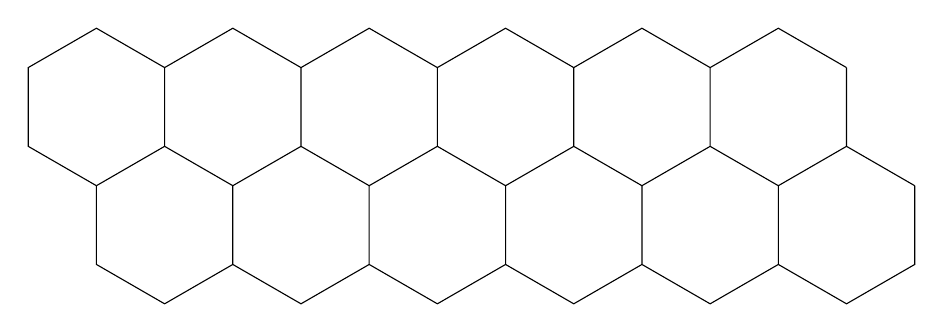
\begin{tikzpicture}
	\draw (0,0) -- ++(90:1) -- ++(-90:1) -- ++(-30:1) -- ++(30:1) -- ++(90:1) -- ++(-90:1) -- ++(-30:1) -- ++(30:1) -- ++(90:1) -- ++(-90:1) -- ++(-30:1) -- ++(30:1)-- ++(90:1) -- ++(-90:1) -- ++(-30:1) -- ++(30:1) -- ++(90:1) -- ++(-90:1) -- ++(-30:1) -- ++(30:1) -- ++(90:1) -- ++(-90:1) -- ++(-30:1) -- ++(30:1) -- ++(90:1);
	\draw (0,1) -- ++(30:1) --  ++(90:1) -- ++(-90:1) --++(-30:1) -- ++(30:1) --  ++(90:1) -- ++(-90:1) -- ++(-30:1) -- ++(30:1) --  ++(90:1) -- ++(-90:1) -- ++(-30:1) --  ++(30:1) --  ++(90:1) -- ++(-90:1) -- ++(-30:1) -- ++(30:1) --  ++(90:1) -- ++(-90:1) -- ++(-30:1) -- ++(30:1) -- ++(90:1) -- ++(-90:1) -- ++(-30:1);

	\draw (0,1) -- ++(150:1) -- ++(0,1) -- ++(30:1) -- ++(-30:1) -- ++(30:1) -- ++(-30:1) -- ++(30:1) -- ++(-30:1) -- ++(30:1)-- ++(-30:1) -- ++(30:1) -- ++(-30:1) -- ++(30:1) -- ++(-30:1);
\end{tikzpicture}
\caption{Infinite Beehive}
\end{figure}

\begin{figure}
\begin{tabular}{|*{8}{c|}} \hline
	$n$ & 1 & 2 & 3 & 4 & 5 & $\dots$ & $n$ \\ \hline
       $b_n$ & 1 & 2 & 3 & 5 & 8 & $\dots$ & $F_n$ \\ \hline
\end{tabular}
	\caption{Number of Paths}
\end{figure}
\end{frame}

\subsection{Fibonacci and Subsets}
\begin{frame}
\frametitle{Fibonacci and Subsets}
\begin{itemize}
	\item The number of subsets (including null set) of a set of $n$ points such that consecutive points are not allowed if the points lie on a line.
		$$ A_1 = 2,\quad A_2 = 3,\quad A_n = A_{n-1} + A_{n-2} = F_{n+2} $$
	\item The number of subsets (including null set) of a set of $n$ points such that consecutive points are not allowed if the points lie on a circle.
	$$ B(1) = 2,\quad B(2) = 3,\quad B(3) = 4$$ 
	$$ B_n = A_{n-1} + A_{n-3} = F_{n+1} + F_{n-1} = L_n $$
\end{itemize}

\end{frame}

\subsection{Fibonacci and Sewage Treatment}
\begin{frame}
\frametitle{Fibonacci and Sewage Treatment}
\end{frame}

\subsection{Fibonacci and Atoms}
\begin{frame}
\frametitle{Fibonacci and Atoms}
\end{frame}

\subsection{Fibonacci and Reflection}
\begin{frame}
\frametitle{Fibonacci and Reflection}
\end{frame}

\subsection{Fibonacci, Paraffins and Cycloparaffins}
\begin{frame}
\frametitle{Fibonacci, Paraffins and Cycloparaffins}
\end{frame}

\subsection{Fibonacci and Music}
\begin{frame}
\frametitle{Fibonacci and Music}
\end{frame}

\subsection{Fibonacci and Compositions with 1`s and 2`s}
\begin{frame}
\frametitle{Fibonacci and Compositions with 1`s and 2`s}
\end{frame}

\begin{frame}
	\vspace{0.6in}
	\hspace{3cm} {\color{blue}\Huge{Thank You}}
\end{frame}
\end{document}
